% Chapter Template

\chapter{Deployment} % Main chapter title

\label{Chapter5} 

\section{Technologies}

There are a lot of IaC solutions out there. Ansible, Terraform, Pulumi, \ldots. 
They all have their own positives and negatives. Choosing the right tool for the job is not easy

Some of the main factors when choosing were

\begin{itemize}
	\item Integration with AWS
	\item Easily scriptable
\end{itemize}

Since Stampix currently runs all their infrastructure on AWS, it makes sense to choose a tool that has good integration with AWS. 
Multiple static site builds will be deployed onto AWS, this means there is some logic involved for each build.
This is why the solution this paper proposes should be easily scriptable: write the infrastructure as code and not as a declarative language (JSON or YML).




\section{AWS CDK}

\begin{quote}
	The AWS Cloud Development Kit (AWS CDK) is an open source software development framework to define your cloud application resources using familiar programming languages.
	\hfill \cite{awscdk}
\end{quote}

I chose AWS CDK because 

\begin{itemize}
	\item it is made by AWS, so the integration with AWS will be great
	\item it allows us to write infrastructure as javascript code
\end{itemize}

Being able to use Javascript is a big bonus since Javascript is the main language used at Stampix. Everyone in the team knows it well.

\section{Configuration}

As mentioned earlier, every static site needs a separate configuration. 
This configuration will determine what client the build is for, allowing us to fetch the right assets from the CMS. 
Furthermore, this configuration will also allow us to enable or disable certain modules. 

In the proof of concept, this configuration is a static JSON document (see the file packages/infra/config.json). This JSON document does not have to be a static file though. 
It could come from the CMS or even a custom application. 
The goal is to make sure that non-technical people can create deployments. This means that they should not be editing straight JSON files.
Instead, the person creating the deployment should be guided through a form in order to create this configuration. 
When submitting this form, a message will be sent to Stampix' CI/CD pipeline to trigger a new build. 

To make this experience as smooth as possible, a good option is creating a custom application to guide the non-technical teammembers in creating these configs. 
However, the implementation of this is outside the scope of this paper

\section{Build and deployment flow}

In order to deploy websites, a domain name is needed. For this, AWS' managed DNS service, Route 53 \footnote{https://aws.amazon.com/route53/} will be used.

The first thing that happens is the configuration JSON is retrieved and read. Based on the contents, several builds of the frontend application are started.

The built files get stored inside S3 \footnote{https://aws.amazon.com/s3/}. Every campaign gets a separate bucket.

The script will also provision TLS certificates via AWS. 
Finally, a CloudFront \footnote{https://aws.amazon.com/cloudfront/} distribution is set up. This will make sure the static files get served when someone visits our sites.

The implementation of this can be found in the directory packages/infra


\begin{figure}[h!]
	\centering
	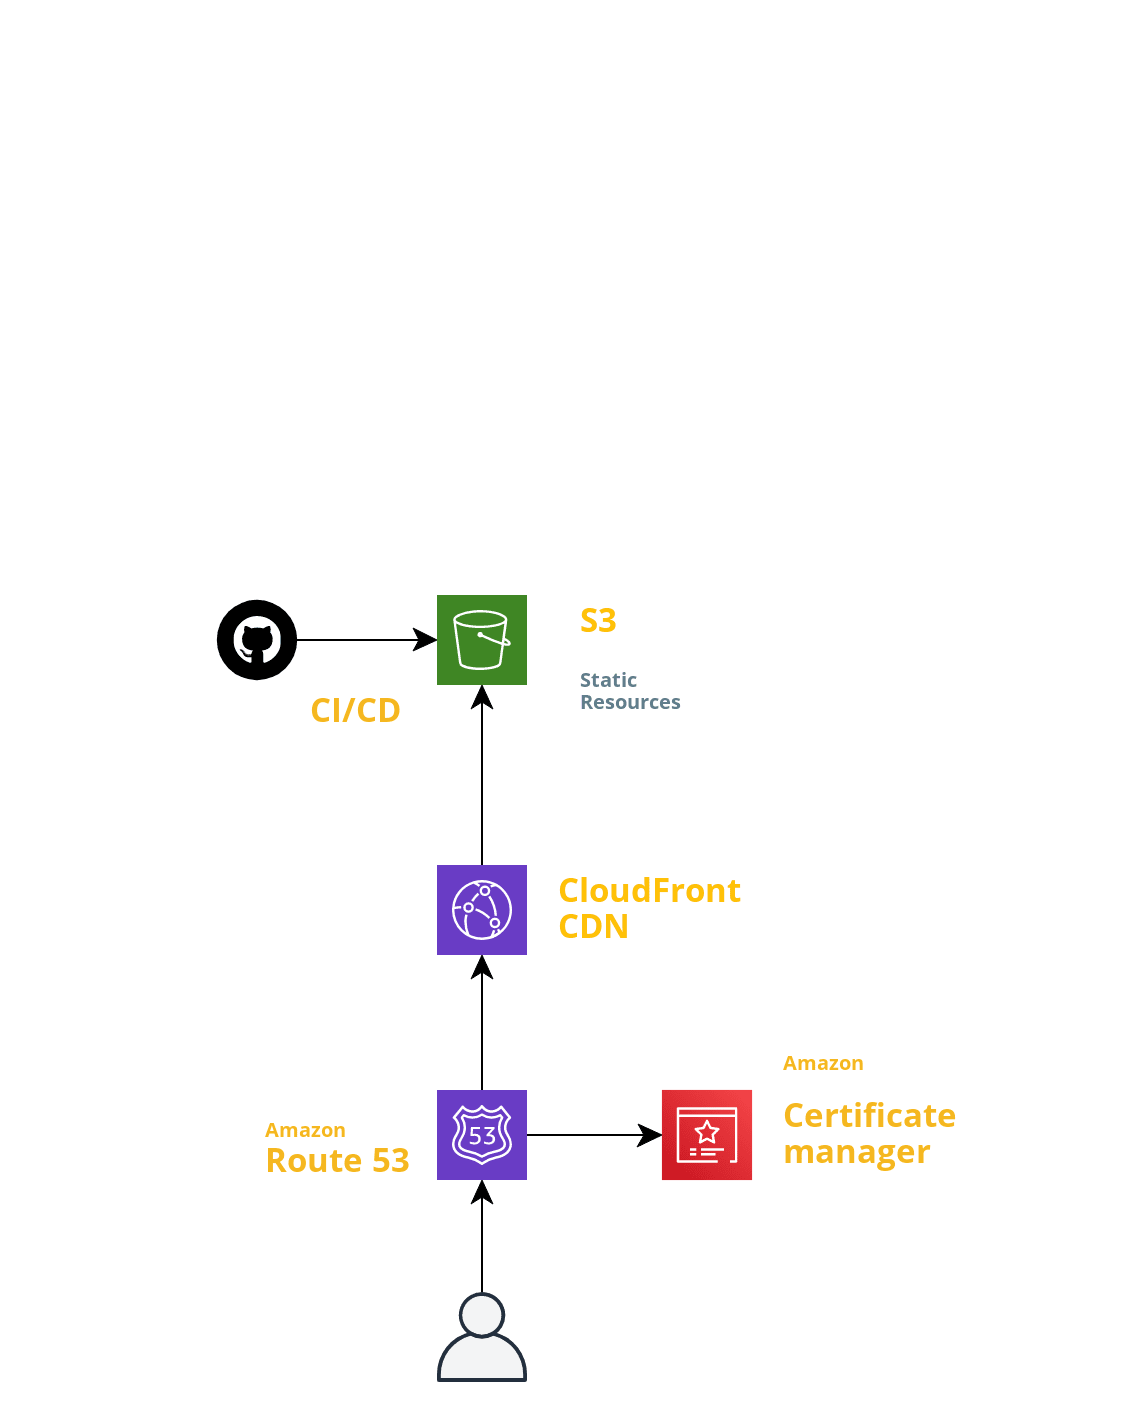
\includegraphics[scale=0.50]{deployment}
	\caption{Final deployment diagram}
	\label{fig:deployment}
\end{figure}